\chapter{Contribution to the DREAM project} \label{app:dream}

As part of DREAM, I have been involved in an international and multidisciplinary project. This lead to numerous meetings and collaboration. While not presented in the main body of this theses, I developed tow tools to automate tasks and contributed to a significant part of the software developed during the DREAM project.

\section{Software development}

The main part of the development was focus on the control architecture for having a robot provide therapeutic sessions for children with \gls{asd}~\citep{esteban2017build}. Workpackage 6 (Plymouth and Vrije Universiteit Brussel) was responsible to develop the cognitive controller of the robot and the different tasks the robot would complete with the child. The overall system used the concepts behind the \gls{sa}, the robot suggest actions to the therapist, and the therapist can cancel them before their execution if their are incorrect. In the case of correct actions, the workload on the therapist is minimal as no correction is required. I developed mostly alone the deliberative, expression and actuation and naoInterface subsystems, The deliberative subsystem was responsible to interpret steps from a script defining the session flow, keep track of the progress in the session and define actions that should be submitted to the teacher. Based on the teacher approval or selection of an action the actuation subsystem selected the correspond primitives to send to the robot. And finally the naoInterface interpreted these general primitives into actions executable by the robot and sent them to the robot for execution. 

Part of the work was also converting scripts provided by the therapist into steps the robot could follow. The initial material provided by the therapists were human defined steps, so these needed to be converted to logic steps that could be used to control the robot. Then, for each unique behaviour requested by the therapist, a corresponding robot behaviour had to created.

\section{Tools}

In addition to the components developed to run the DREAM application, I created two tools. The first one automated and simplified the use of the YARP middleware while conforming to the development standards imposed on the project, and the second one provided a human interface to create and modify the scripts used in the therapy sessions.

\subsection{yarpGenerator}

The software development guidelines of DREAM imposed a specific structure for folders of new components developed with a number of constant part throughout the required 6 files. Additionally, adding or removing one port required changes in 5 files in more than 10 location. To ease this procedure, I proposed to add two new class: the yarpInterface and the yarpController. yarpInterface class exposes all the yarp output ports required by the component to C++ function and integrates callbacks asynchronously called when messages arrive on input ports. And the yarpController corresponds to a C++ only file where the code can be developed without reliance on YARP. This class (and others) can call functions from yarpInterface to send messages and be called by callbacks in yarpInterface to react to messages. The yarpGenerator is a tool generating automatically compilable code, complient with the development standards and including all the required files and the code to have ports working. Appendice~\ref{app:yarpgenerator} presents the techreport created to describe the tool.

\subsection{scriptManager}

The second tool provided a graphical way to read and edit the xml files describing the scripts used in the therapies. No technical report is available for this tool.

\cleartooddpage
\chapter{Social Assistive Robot for Cardiac Rehabilitation} \label{app:yarpgenerator}
This appendix section presents the technical report corresponding to the yarpgenerator tool created for DREAM.

\foreachpage{appendices/yarpgenerator-guidelines.pdf}{%
	\newpage   
	\begingroup 
	\centering
	\includegraphics[
	page=\value{imagepage},
	width=\textwidth,  
	height=\textheight,
	keepaspectratio,
	]{appendices/yarpgenerator-guidelines.pdf}%
	\newpage
	\endgroup
}


\cleartooddpage
\chapter{Social Assistive Robot for Cardiac Rehabilitation} \label{app:Colombia}

A  second project I was involved in during this research work was a collaboration with the Escuela Colombiana de Ingeniería Julio Garavito in Bogota. This project:  the Human-Robot Interaction Strategies for Rehabilitation based on Socially Assistive Robotics project (Royal Academy of Engineering: IAPP\textbackslash1516\textbackslash137) aimed at developing a social robot to support, monitor and assist cardiac rehabilitation for patient affected or susceptible to suffer from cardiovascular disease.

During that project, my role was to design the robot's behaviour: guiding the patients through the therapy, providing encouragements or feedback on their postures (through their head gaze and position on the treadmill) and monitoring their signals. Using preprocessed inputs from sensors (such as heartbeat or level on a pain scale) and rules from the therapists, the robot also had to request help if the patient was in a bad situation. So far this collaboration contributed to two publications~\citep{lara2017human,casas2018social}, but more should be arriving in the coming months.

\cleartooddpage
\chapter{Teacher's Diary} \label{app:diary}
This appendix section presents the daily report of the teacher's impressions and feeling when teaching the robot in the study in Chapter\ref{chap:tutoring}. It should be noted that among all the children supervised, many were special needs and as such have been removed from the result analysis. This also explains the difference of number between the children in the supervised condition (n=25) and in this diary (n=34).

%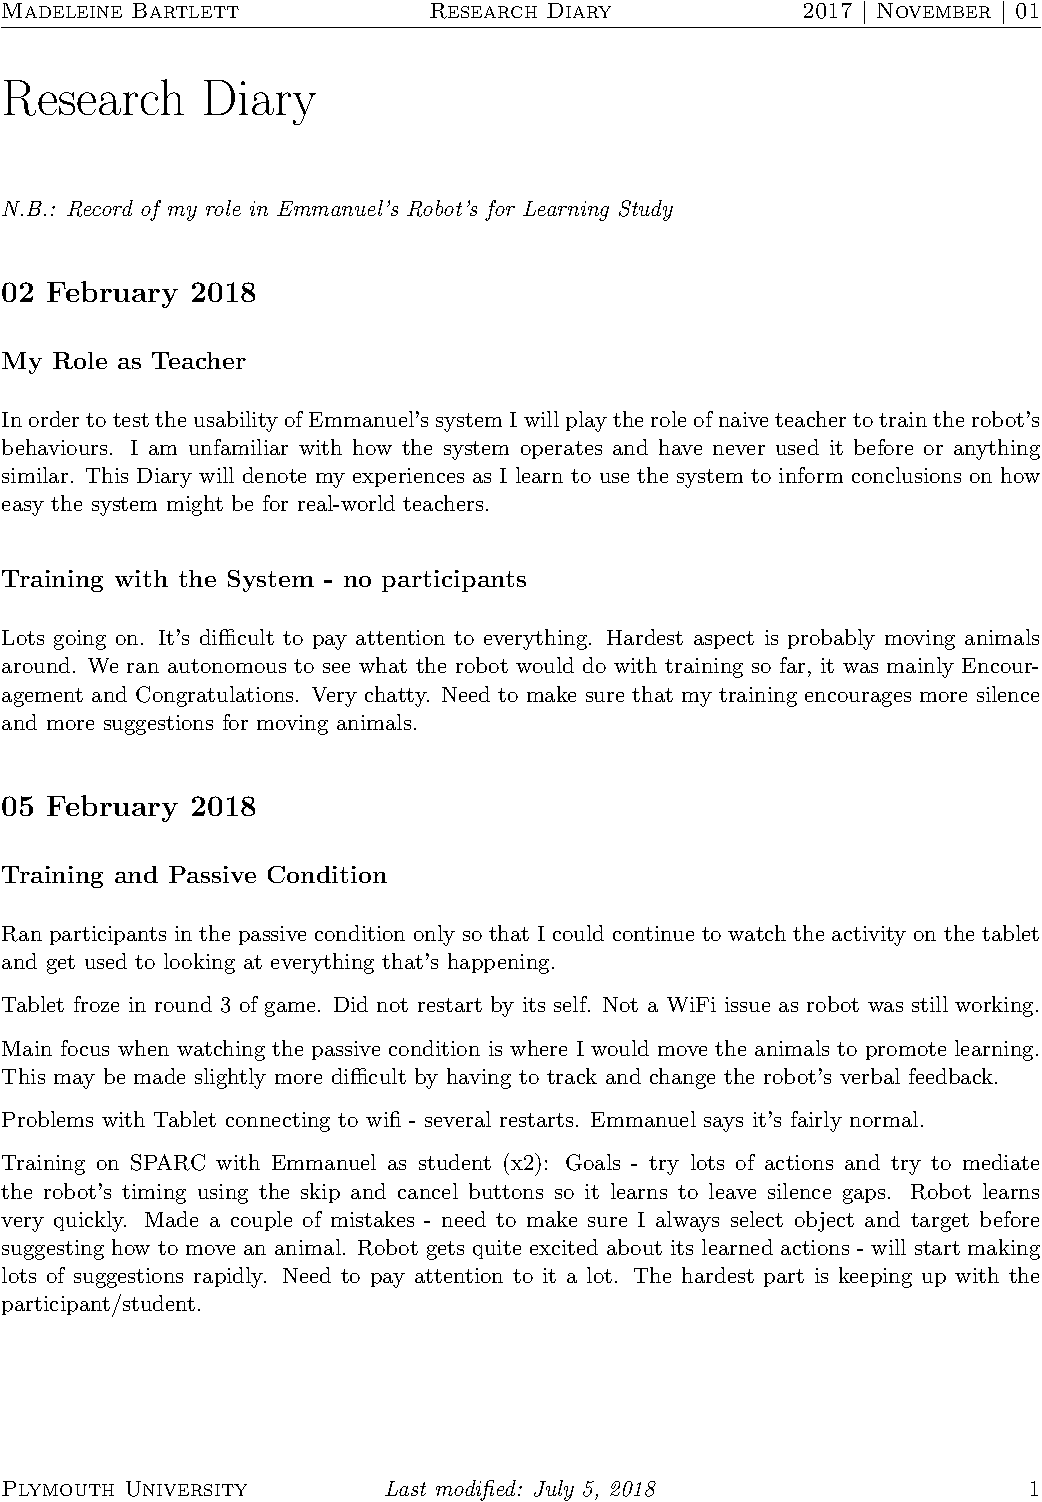
\includepdf[pages=1-14,pagecommand={},linktodoc=true]{appendices/research-diary.pdf}
\foreachpage{appendices/research-diary.pdf}{%
	\newpage   
	\begingroup 
	\centering
	\includegraphics[
	page=\value{imagepage},
	width=\textwidth,  
	height=\textheight,
	keepaspectratio,
	]{appendices/research-diary.pdf}%
	\newpage
	\endgroup
}